% 第4章：课程课件与教材核对后整理；图示来源见 Book/page_index.md。
\chapter{网络层}
\noindent\textbf{本章要解决的问题。} 第3章解决相邻结点之间怎样传递帧；网络层解决怎样把分组跨过多个不同网络，从源主机送到目的主机。为此，网络层需要地址、转发表以及建立转发表的路由协议；还要处理分组过大、地址配置和差错报告等问题。本章依照课件顺序展开。

\small 本章来源页码写作“PDF阅读器页（课件显示页）”；两者相同时只列一个页码。教材页码均注明PDF页和印刷页，不能互换。\normalsize

\section{网络层服务}
\subsection{转发、路由与服务模型}
主机发送时将传输层的报文段等数据封装为\textbf{IP数据报}，经过多个路由器，到达目的主机后交给相应上层协议。路由器通常不需要知道应用内容，而依据分组首部及转发表决定如何处理。网络层的工作可分为\textbf{数据平面}和\textbf{控制平面}：数据平面逐个处理数据报，控制平面决定各路由器应使用哪些转发表项。传统路由协议由多个路由器协同计算；课件也简要介绍由控制器集中计算规则的SDN思路。

\textbf{转发（forwarding）}是单个路由器收到分组后，将其从输入接口送往合适输出接口的动作；\textbf{路由选择（routing）}是根据拓扑和规则确定到达目的网络的路径、形成路由信息的过程。可把前者理解成路口按路牌选择出口，后者是如何确定和更新路牌。路由表侧重路径计算，转发表是为高速查找整理出的结果；简化讨论时两者常统称路由表。

互联网的网络层通常提供\textbf{无连接、尽力而为}的数据报服务：发送前不由网络层为该数据流建立连接，网络尽力传递但不保证送达、按序、无重复或特定时延。若应用需要可靠交付，可由 TCP 等上层机制提供。网络层服务是主机到主机；传输层面向应用进程，TCP 的连接由端系统维护，并不要求中间路由器建立 TCP 连接状态。

\subsection{拥塞及其代价}
\textbf{拥塞}指注入网络的流量超过某些链路或设备的处理能力。有限缓存排满会丢包；即使缓存很大，等待时间也会增长。发送方重传会占用更多链路能力；一包已走过多跳后才丢失，之前各跳消耗的资源也不能收回。拥塞控制关注整个网络的负荷，\textbf{流量控制}主要防止某个接收方来不及接收，两者目的不同。

拥塞可以由端系统根据丢包、时延等迹象推测，也可以由网络设备显式反馈。课件介绍的网络辅助手段包括流量感知路由、准入控制、调节发送流量与过载时主动丢弃；ATM ABR 服务使用资源管理信元反馈拥塞或可用速率。这些是不同体系的机制，不代表 IP 本身承诺固定速率。\par\small\noindent 来源：第4章课件 PDF 第4--18页；参考书 PDF 第138--143页（印刷第127--132页）。\normalsize

\annotationarea[4]
\section{虚电路网络与数据报网络}
\textbf{虚电路（VC）}是分组交换网络中的逻辑路径。典型过程为建立、沿路径传输、拆除；建立时路径上的设备保存状态。一个分组携带本段链路有效的虚电路号 VCID，路由器用“输入接口、输入 VCID”查表，得到“输出接口、输出 VCID”，然后替换编号。不同链路上同一虚电路的编号可以不同；它仍共享物理链路，不等于独占电路，是否预留带宽及可靠性取决于具体服务。

\begin{figure}[H]\centering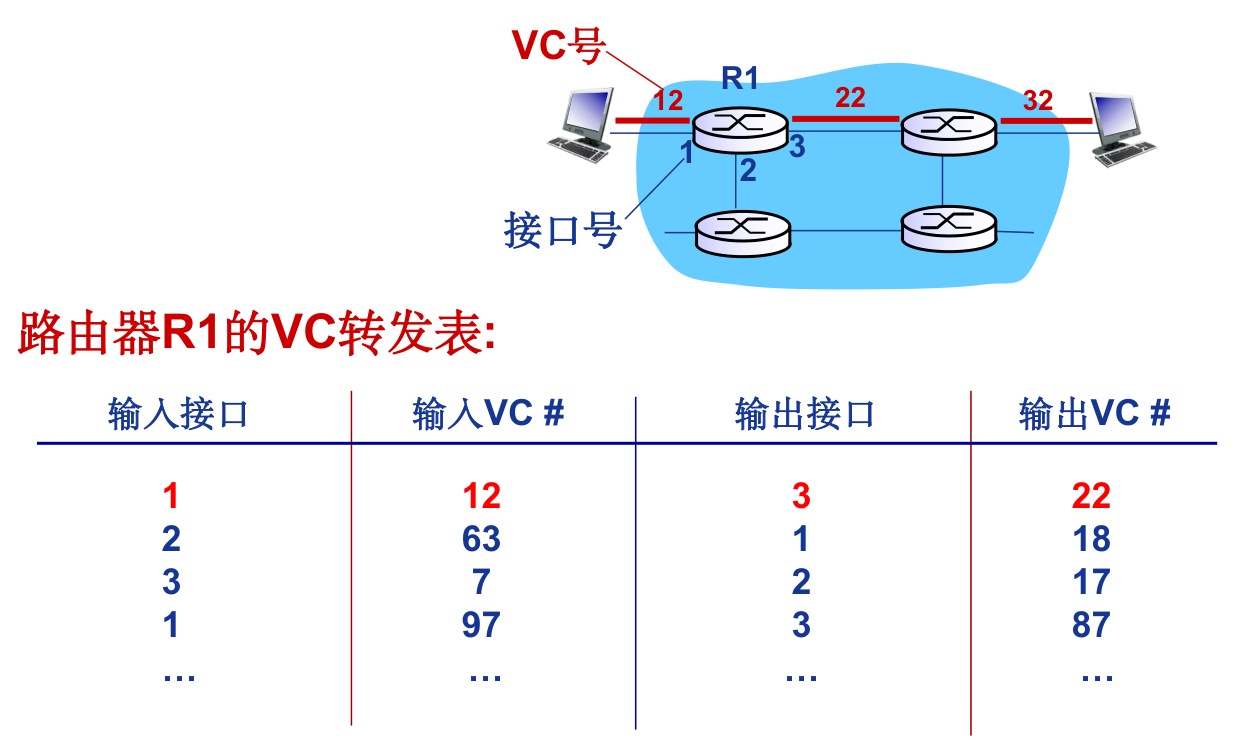
\includegraphics[width=.83\textwidth]{ch04-vc-table.png}\caption{虚电路转发表：输入接口1、编号12对应输出接口3、编号22。来源：Chapter4-网络层.pdf，PDF第24页（显示页24），局部截取。}\end{figure}

\textbf{数据报网络}不为一串数据报预先建立网络层连接。每个分组携带目的地址，路由器对它独立查表；在路由变化时同一应用的分组可能走不同路径。不同路径、排队和丢包都可能使分组失序。与 VC 不同，普通 IP 路由器不按每个用户会话保存连接状态。

\textbf{最长前缀匹配。} 前缀是地址的前若干位。若目的地址同时匹配多条路由，选共同前缀最长的一条；例如 \texttt{200.23.24.5} 同时匹配 \texttt{200.23.0.0/16} 和 \texttt{200.23.24.0/24}，选择后者。默认路由 \texttt{0.0.0.0/0} 只有在没有更具体匹配时使用。若既无匹配又无默认路由，则无法按表继续转发。
\par\small\noindent 来源：课件 PDF 第20--33页；教材 PDF 第140--142页（印刷第129--131页）。\normalsize

\annotationarea[4]
\section{路由器体系结构}
路由器包括运行路由协议、管理路由信息的\textbf{路由处理器}，以及高速处理分组的输入端口、\textbf{交换结构}和输出端口。输入端口接收信号、处理链路层帧、查询转发表；交换结构把分组移向对应输出；输出端口排队、选择发送顺序，重新封装并送往下一条链路。
\begin{figure}[H]\centering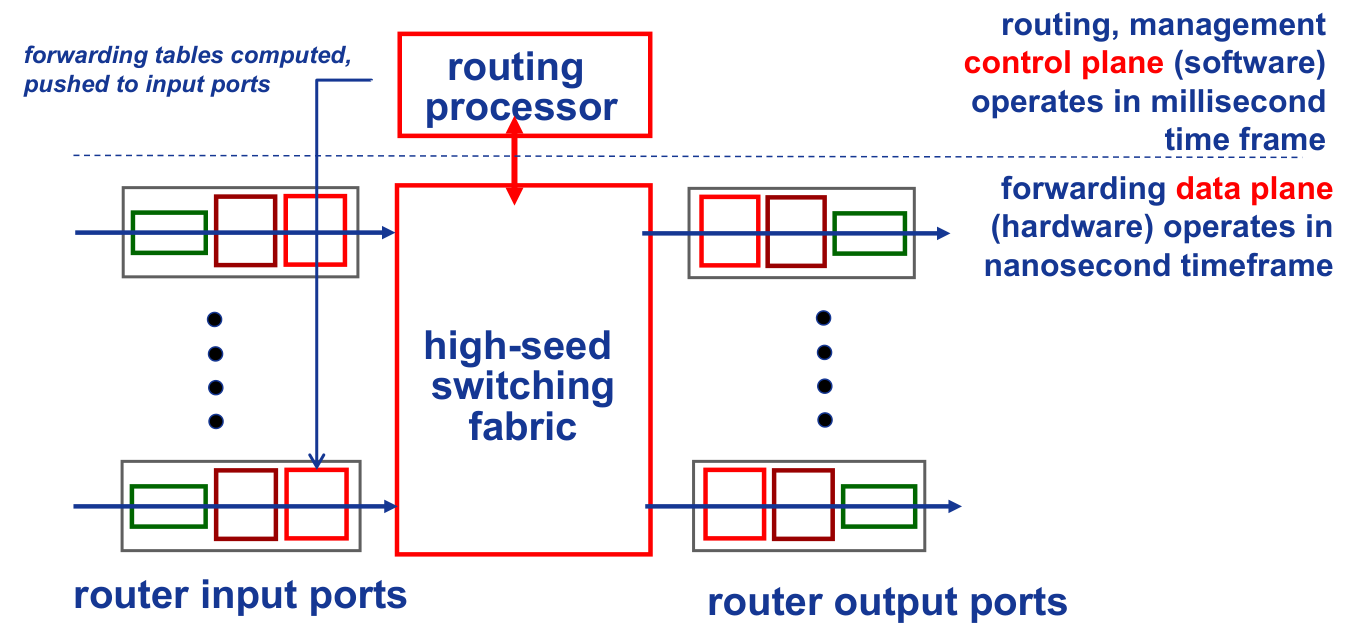
\includegraphics[width=.8\textwidth]{ch04-router.png}\caption{路由器内部：左侧输入端口经交换结构连接右侧输出端口，处理器提供转发所需的表。来源：Chapter4-网络层.pdf，PDF第35页（显示页35），局部截取。}\end{figure}
交换结构可以通过共享内存、共享总线或互连网络实现；前两者受共享带宽制约，交叉开关等互连结构可允许不同输入到不同输出并行。输入到达速率高于交换结构处理能力时，输入处排队；队首分组争不到输出而阻挡后面本可发送的分组，称\textbf{队首阻塞}。若多个输入同时汇聚到同一输出，输出链路来不及发送也会排队，缓存满则丢包。

\textbf{调度}决定等待分组的发送顺序：FIFO 先到先服务；优先级调度先选高优先级，低优先级可能长期等待；轮询依次服务各类队列；加权公平排队按权重分配服务，所有队列持续有待发数据时，可近似按权重分享链路，实际分组长度会影响瞬时顺序。课件给出的按带宽与 RTT 估算缓存容量是经验模型，适用前提决定其结果，不能当成固定标准。\par\small\noindent 来源：课件 PDF 第35--51页；教材 PDF 第225--227页（印刷第214--216页）。\normalsize

\annotationarea[4]
\section{IP协议}
\subsection{IPv4首部与逐跳处理}
IPv4 地址长32位，写作四个0--255的十进制数，例如 \texttt{192.168.1.10}。数据报由首部和数据组成；首部至少20字节，携带目的地址和各项处理信息。
\begin{figure}[H]\centering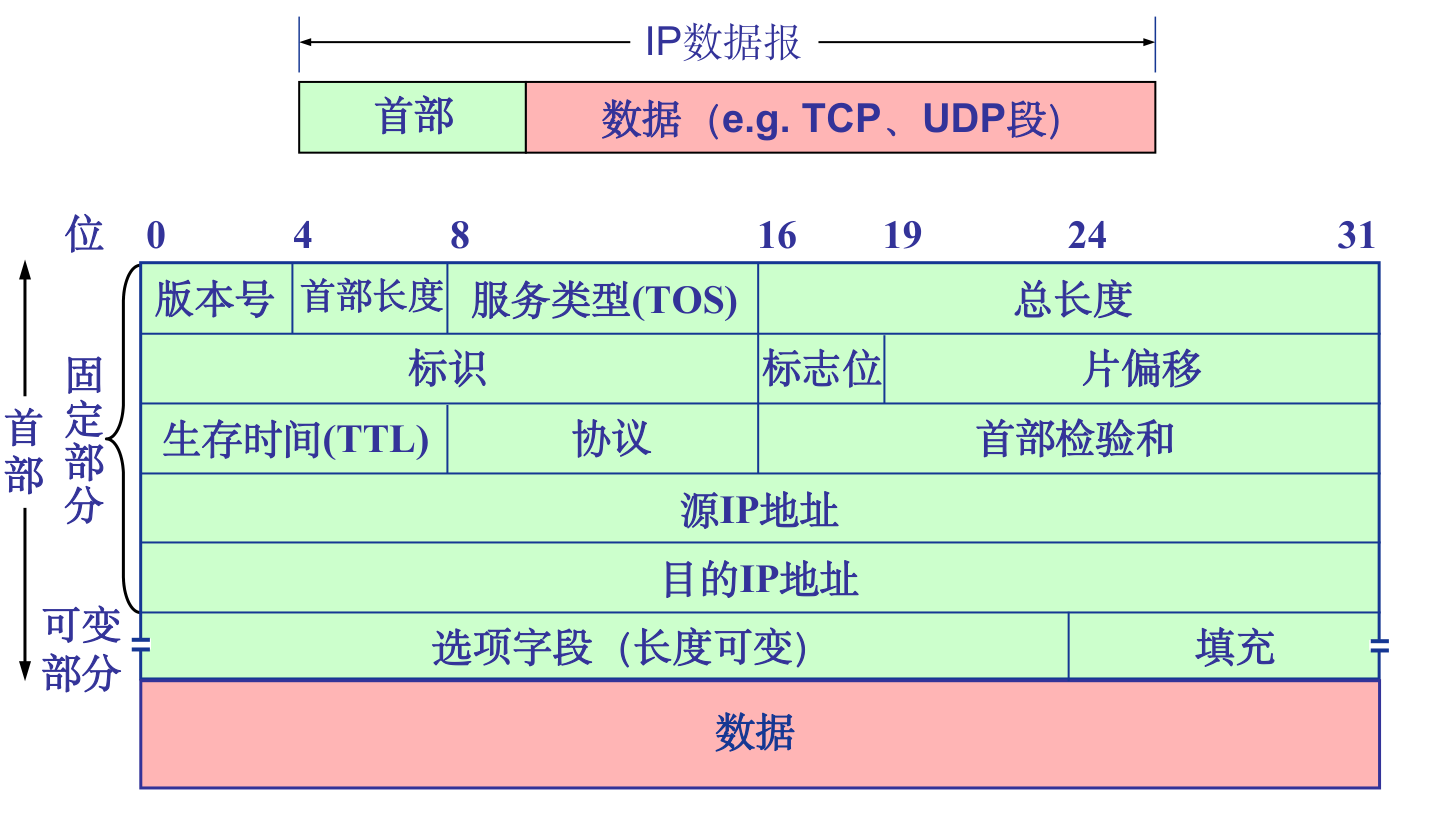
\includegraphics[width=.83\textwidth]{ch04-ipv4-header.png}\caption{IPv4数据报首部与载荷；横向字段宽度之和每行为32位。来源：Chapter4-网络层.pdf，PDF第54页（显示页54），局部截取。}\end{figure}
\begin{itemize}[nosep]
\item \textbf{版本}4位，IPv4取4；\textbf{首部长度 IHL}4位，以4字节为单位，因此值5表示20字节，最大值15表示60字节。选项使首部可变长，填充用于4字节对齐。
\item \textbf{服务类型}8位，现代解释包括DSCP和ECN；\textbf{总长度}16位，以字节计，包含首部和载荷，最大65535字节。
\item \textbf{标识}16位；\textbf{标志}3位；\textbf{片偏移}13位。DF=1表示不允许分片；MF=1表示后面还有分片；片偏移单位为8字节。
\item \textbf{生存时间 TTL}8位，在每个转发路由器递减，减至0则丢弃以限制环路；\textbf{协议}8位，指出载荷交给哪种上层协议，如ICMP=1、TCP=6、UDP=17。
\item \textbf{首部校验和}16位，只检验IPv4首部，不检验载荷；TTL等字段改变时须更新。源、目的IP各32位；普通路由转发通常不改它们，NAT等特殊处理会改写。
\end{itemize}

\subsection{MTU与IPv4分片}
\textbf{最大传输单元（MTU）}是当前链路能够承载的最大IP数据报长度，含IP首部而不含链路帧首尾。若数据报长于输出链路MTU，IPv4路由器在DF=0时可以分片；DF=1则丢弃并可返回相应ICMP差错。片由目的主机重组，一个片丢失会使原数据报无法完整重组。

\textbf{课件例：}原报总长4000字节，首部20字节，无选项，MTU=1500字节。原载荷 $4000-20=3980$ 字节；前两片载荷各1480字节，均为8的倍数；余下 $3980-2960=1020$ 字节。每片都要重新拥有20字节首部：
\begin{center}\begin{tabular}{cccc}\toprule 片 & 总长（字节） & MF & 片偏移（8字节）\\\midrule 1 &1500&1&0\\2&1500&1&185\\3&1040&0&370\\\bottomrule\end{tabular}\end{center}
片偏移是相对于\emph{原数据载荷起点}，例如第二片从第1480字节开始，所以偏移为 $1480/8=185$；所有片标识相同。除最后一片外，载荷长度须为8的倍数。若首部长度或选项复制情况不同，应按各片实际首部重新计算，不能机械套用20字节。若已经是分片的数据报再次分片，新片偏移须在原片偏移基础上计算；原片MF为1时，产生的最后一小片也仍须标记MF=1。
\begin{figure}[H]\centering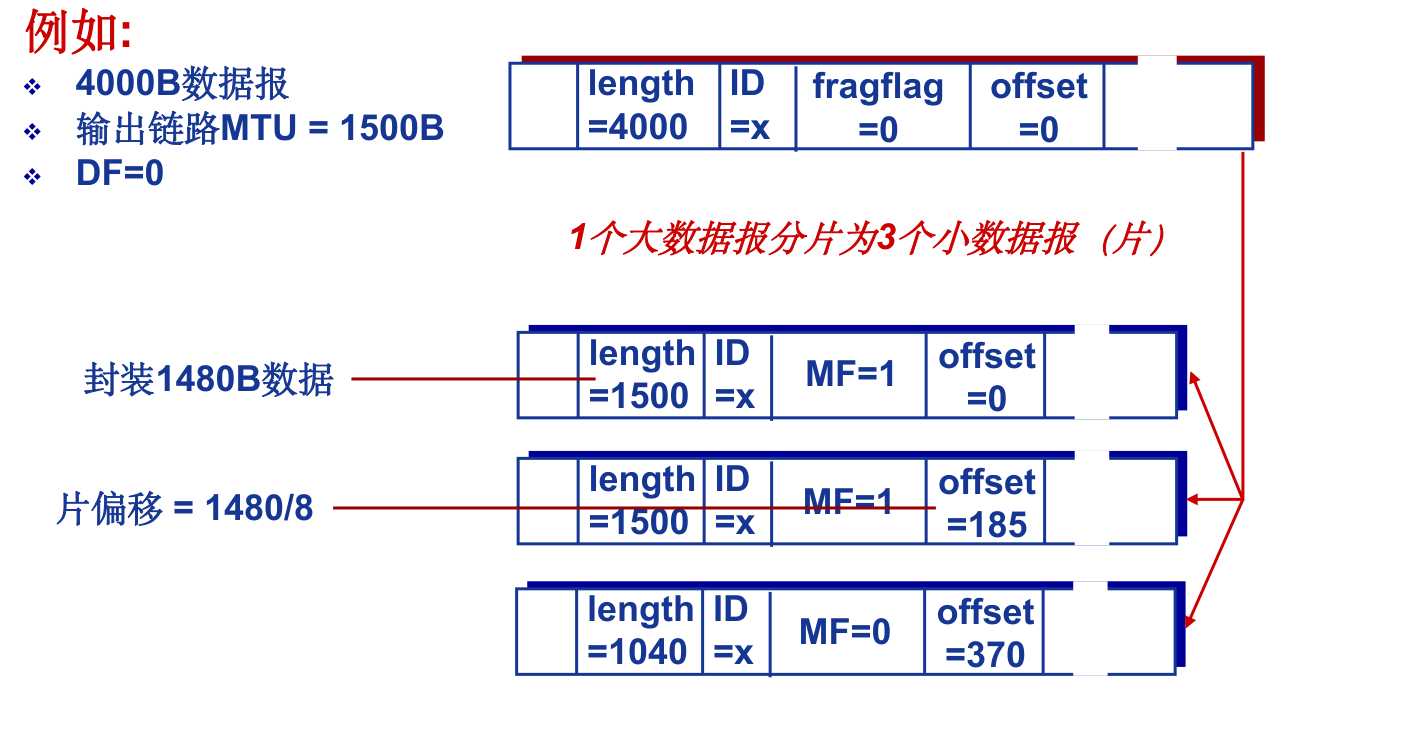
\includegraphics[width=.86\textwidth]{ch04-fragments.png}\caption{4000字节IPv4数据报的分片过程；箭头表示由原报产生三个独立IP分片。来源：Chapter4-网络层.pdf，PDF第72页（显示页72），局部截取。}\end{figure}

\subsection{地址、子网、掩码与无类编址}
IP地址通常配置在接口上，路由器连接多条网络，因而各接口可有不同地址。子网中地址高位的\textbf{网络前缀}相同，低位区分接口；路由器借前缀找到目标网络。\textbf{掩码}是前缀位为1、余下为0的32位数，地址与掩码逐位做 AND，得到网络地址。\texttt{/23} 表示前23位为前缀，即掩码 \texttt{255.255.254.0}。

\begin{sloppypar}
\textbf{课件例：}地址 \texttt{172.32.1.112/23} 中第三字节 $1=00000001_2$，掩码第三字节 $254=11111110_2$；与运算为0，因此网络为 \texttt{172.32.0.0/23}。主机部分9位，地址共 $2^9=512$ 个：从 \texttt{172.32.0.0} 到 \texttt{172.32.1.255}。对于普通广播子网，首地址表示网络、末地址为定向广播地址，可分配范围为 \texttt{172.32.0.1} 至\allowbreak \texttt{172.32.1.254}，共510个。点到点 /31 与主机路由 /32 有特殊用途，不能套用减2公式。
\end{sloppypar}

历史上的A、B、C类默认前缀分别为8、16、24位；D类用于多播，E类保留。A类0和127等范围有特殊用途，不能简单认为每个地址都可作普通主机地址。现在常用\textbf{无类域间路由 CIDR}，用地址加前缀长度指明范围；私有地址为 \texttt{10.0.0.0/8}、\texttt{172.16.0.0/12}、\texttt{192.168.0.0/16}，不应在公共互联网按普通公网地址转发。

\textbf{课件划分例：}将 \texttt{192.168.1.0/24} 中已分配的 \texttt{192.168.1.0/25} 留出后，剩余 \texttt{192.168.1.128/25} 划分给需要60、30、30个地址的三个局域网。先分最大需求：/26有64个地址、62个可分配；两个/27各有32个地址、30个可分配：
\begin{center}\begin{tabular}{llll}\toprule 前缀 & 可用地址范围 & 广播地址 & 可用数\\\midrule
192.168.1.128/26 & .129--.190 & .191 & 62\\
192.168.1.192/27 & .193--.222 & .223 & 30\\
192.168.1.224/27 & .225--.254 & .255 & 30\\\bottomrule\end{tabular}\end{center}
表中简写的末字节均属于 \texttt{192.168.1}。分配地址应先选能容纳需求的最小块，并按块边界对齐，确认各块不重叠。

\begin{sloppypar}
\textbf{路由聚合}用一个共同前缀概括多个目的网络，缩小路由表。例如相邻的\allowbreak \texttt{202.118.1.0/25} 与\allowbreak \texttt{202.118.1.128/25} 都从同一下一跳可达，可聚合为 \texttt{202.118.1.0/24}。聚合后须检查所有被涵盖地址都能正确转发，否则可能产生黑洞；更具体路由可通过最长前缀匹配覆盖汇总路由。
\end{sloppypar}

\subsection{IPv6与过渡}
IPv6使用128位地址，常写成8组十六进制数；每组前导零可省略，连续全零组可用一次 \texttt{::} 压缩，如 \texttt{FF01::43}。前缀仍用斜线长度表示，例如 \texttt{2002:43c:476b::/48}。单播是一对一，多播是一对多，任播将同一地址分配给一组接口并交付其中一个，通常按路由意义上的最近者选择。

IPv6基本首部固定40字节，有版本、流量类别、流标签、载荷长度、下一个首部、跳数限制、源与目的地址；扩展首部串联可选信息。基本首部没有IPv4首部校验和，路由器不执行IPv6分片；源节点可在需要时使用分片扩展首部。IPv6不使用IPv4式广播。\textbf{隧道}可将完整IPv6数据报装入IPv4载荷穿越IPv4网络，另一端解封装；内外层地址分别服务于原始通信和隧道两端。\par
\textbf{课件中的特殊IPv4地址：}
\begin{center}\small\setlength{\tabcolsep}{4pt}
\begin{tabularx}{\textwidth}{>{\raggedright\arraybackslash}p{5.8cm}>{\raggedright\arraybackslash}X}
\toprule 地址特征 & 课件所述用途\\\midrule
网络号全0、主机号全0 & 本网范围表示本机；在路由表中也可表示默认路由（需看使用场景）\\
网络号全0、主机号为特定值 & 表示本网内某个特定主机\\
网络号和主机号全1 & 本网广播地址，路由器不转发\\
特定网络号、主机号全0 & 网络地址，标识一个网络\\
特定网络号、主机号全1 & 该网络的直接广播地址\\
首字节为127、主机号非全0/全1 & 环回地址，用于本机软件测试\\\bottomrule
\end{tabularx}\end{center}
私有地址范围为\texttt{10.0.0.0/8}、\texttt{172.16.0.0/12}、\texttt{192.168.0.0/16}。\par\small\noindent 来源：课件 PDF 第53--113、201--208页；教材 PDF 第148--154、192--195页（印刷第137--143、181--184页）。\normalsize

\annotationarea[4]
\section{IP相关协议}
\subsection{ICMP、ping与traceroute}
\textbf{ICMP}（Internet控制报文协议）的报文装在IP数据报中，用于报告差错或网络探询，并不使IP传输自动可靠。例子有目的不可达、超时、重定向、回声请求和回声应答；课件所列源抑制是历史机制，不宜当成当前拥塞控制方案。

\textbf{ping}发送回声请求，收到回声应答可测往返时间；无应答可能是丢包或过滤，并不必然说明主机不存在。\textbf{traceroute}逐次发送TTL为1、2、3等的探测报文：第一跳将TTL减至0并可能返回ICMP超时，第二次由第二跳返回，以此推测路径。课件示例采用UDP探测，目的主机可用端口不可达响应终止；不同实现也可能用其他探测报文，路由或过滤变化会使结果不完整。通常不会针对ICMP差错报文再生成ICMP差错，也不会对非首个分片生成ICMP差错。

\subsection{DHCP：自动配置}
\textbf{动态主机配置协议 DHCP}让新加入的主机获得地址、子网掩码、默认网关、DNS服务器及租期。典型初始流程称DORA：
\begin{enumerate}[nosep]
\item 客户端广播 Discover 寻找服务器，尚无地址时源IP为 \texttt{0.0.0.0}；
\item 服务器返回 Offer，提出可用地址及租期；
\item 客户端广播 Request，表示选择某份提供；
\item 被选服务器返回 ACK 确认，客户端才使用配置；租期到期前可以续租。
\end{enumerate}
DHCP采用UDP，服务器端口67、客户端端口68。若服务器不在本广播域，可以通过DHCP中继转发请求；服务器响应不一定总是广播。默认网关是本子网上可转发到其他网络的路由器接口。

\annotationarea[3]
\subsection{NAT：多个内部主机共享外部地址}
\textbf{网络地址转换 NAT}可将内部私有地址与公网地址对应；课件例子同时转换传输层端口，这种多对一形式也称NAPT。主机 \texttt{10.0.0.1:3345} 访问 \texttt{128.119.40.186:80} 时，网关将源改为 \texttt{138.76.29.7:5001}，记录映射；回复以 \texttt{138.76.29.7:5001} 为目的到达网关后，再改回 \texttt{10.0.0.1:3345}。端口帮助区分内部会话，转换还涉及相关校验和更新。
\begin{figure}[H]\centering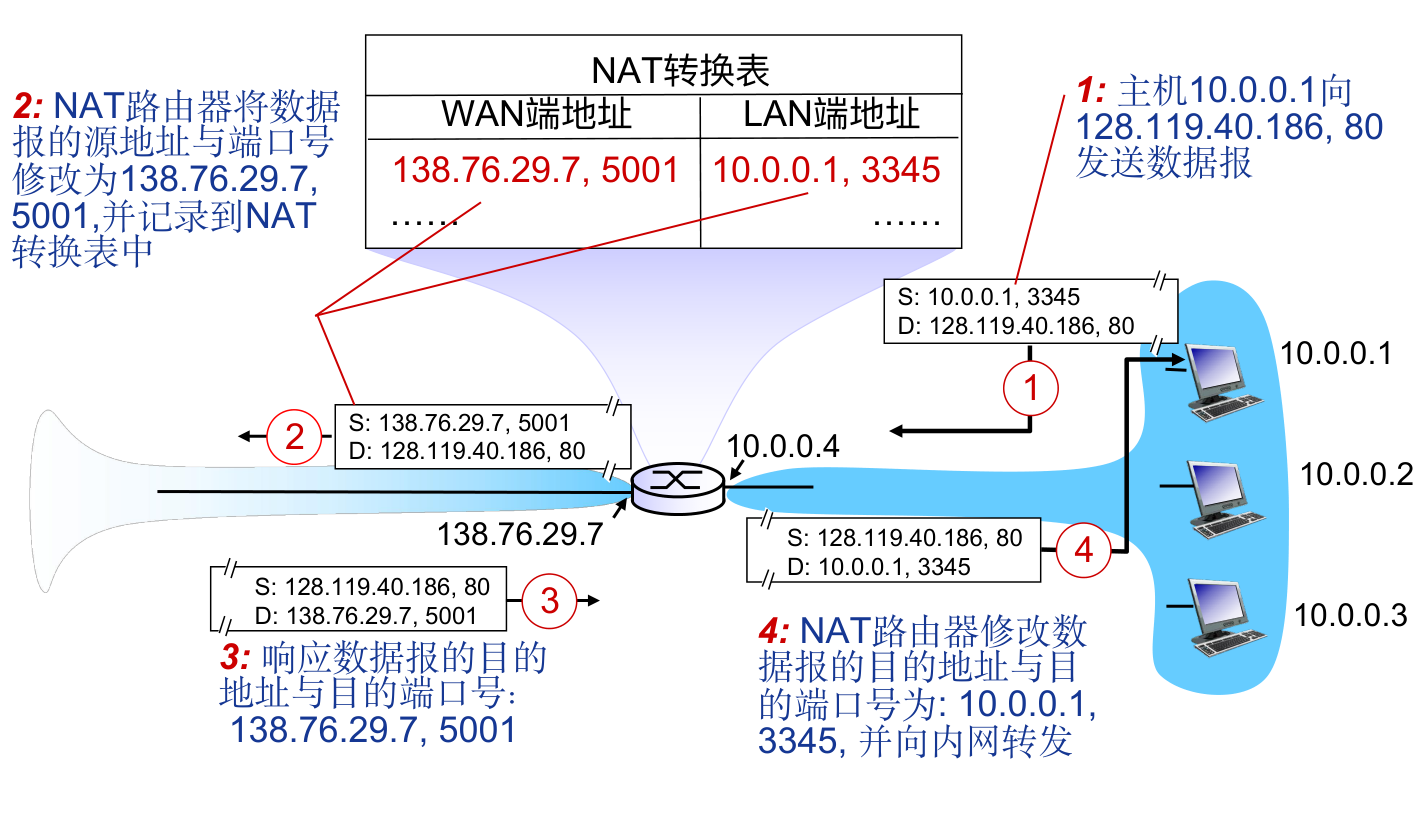
\includegraphics[width=.88\textwidth]{ch04-nat.png}\caption{NAT往返转换：编号1--4依次是请求、改写外出、回复和改写进入，表中记录地址与端口对应。来源：Chapter4-网络层.pdf，PDF第130页（显示页130），局部截取。}\end{figure}
外部主动访问内网服务器时，若没有对应映射，网关通常无法知道转给谁；可配置端口映射、通过网关控制协议建立映射，或使用中继。NAT改变端到端寻址，不等同于完整防火墙或安全保证。

\annotationarea[3]
\subsection{ARP与跨网段逐跳交付}
\textbf{地址解析协议 ARP}在本地链路上把下一跳IPv4地址解析成链路层MAC地址。A需要向同一局域网中的B发报而缓存无记录时，广播询问“谁拥有B的IP”；B通常单播应答其MAC，A缓存映射并设置有效期。ARP广播限制在本地广播域，不跨路由器查找远端主机。

若A与B不在同一子网，A查询到默认网关的IP，再用ARP解析\emph{网关接口}的MAC。第一跳帧的源MAC为A、目的MAC为网关；其中IP数据报源、目的仍为A、B。路由器去除旧帧、查表、解析下一跳并构造新帧；新帧中的MAC因链路而变，而普通转发中端到端IP不变，TTL递减。图中R左右接口各自连接一个网络，蓝色线表示对应链路，帧的目的MAC是本跳接收接口。
\begin{figure}[H]\centering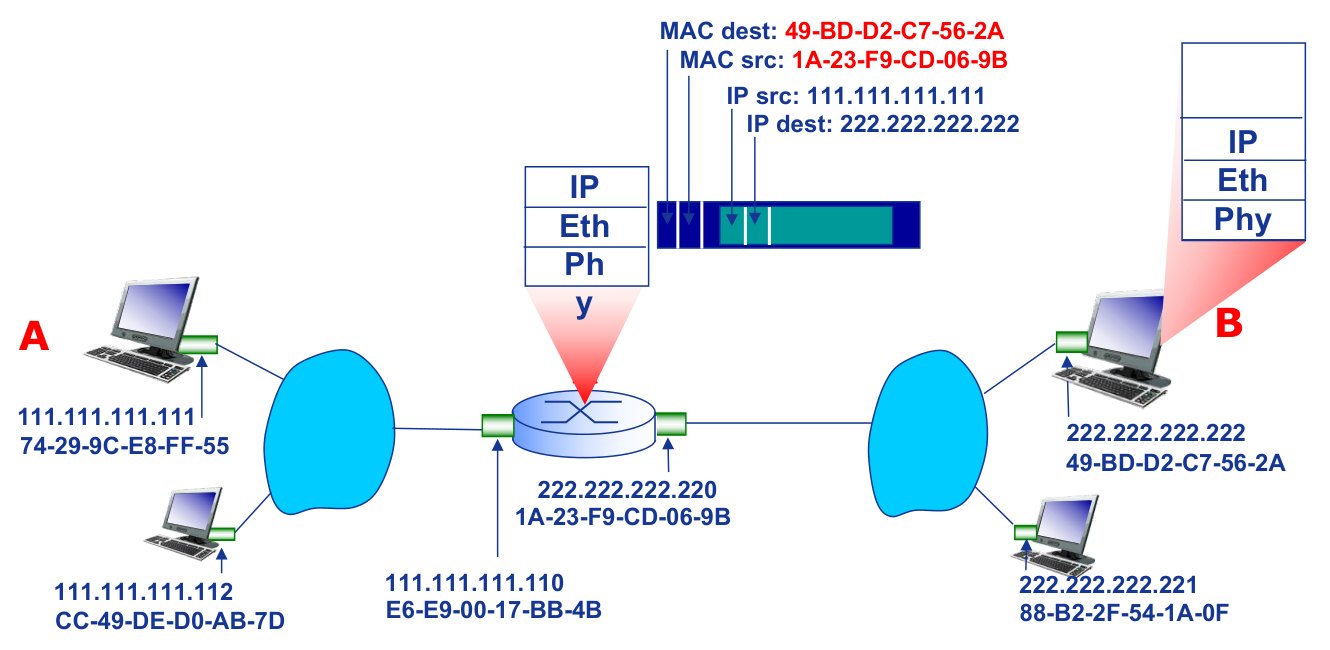
\includegraphics[width=.88\textwidth]{ch04-hop-addresses.png}\caption{跨两个局域网交付：路由器向右转发时，数据报目的IP仍为B，输出帧目的MAC换成B的MAC。来源：Chapter4-网络层.pdf，PDF第145页（显示页145），局部截取。}\end{figure}
\par\small\noindent 来源：课件 PDF 第115--146页；教材 PDF 第155--162页（印刷第144--151页）。\normalsize

\annotationarea[4]
\section{路由算法}
\subsection{图、费用和最短路径}
把路由器抽象为结点、链路抽象为边；链路费用 $c(x,y)$ 可表示跳数、配置的代价等。路径费用是各链路费用之和，\textbf{最短路径}即总费用最小，不一定是物理距离最短。静态路由由管理者配置，动态路由依据协议交换信息并更新；优先级取决于设备具体配置。

\subsection{链路状态与Dijkstra算法}
链路状态算法让路由器通告本地链路信息，参与者形成拓扑图，再各自计算到各目的地的最小费用路径。Dijkstra算法假设链路费用非负；记 $N'$ 为已确定最短费用的结点集，$D(v)$ 为源到结点 $v$ 的当前最好估计。初始化源结点加入 $N'$，其邻居估计设为直接链路费用，其他为无穷。然后重复：
\begin{enumerate}[nosep]
\item 在未确定结点中选 $D$ 最小的结点 $w$，加入 $N'$；
\item 对其未确定邻居 $v$，比较旧路径与经 $w$ 的路径，更新
\[D(v)\leftarrow\min\{D(v),\ D(w)+c(w,v)\};\]
\item 记录前驱，直到目标已确定或所有可达结点确定；沿前驱回溯即可找到源的下一跳。
\end{enumerate}
\textbf{课件图示例：}从 $u$ 出发，直接到 $w$ 的费用3、到 $x$ 为5、到 $v$ 为7。先确定 $w$，经 $w$ 可把 $v$ 改为 $3+3=6$；再确定 $x$，之后确定 $v$，经 $v$ 将 $y$ 更新为10；经 $y$ 将 $z$ 更新为12。表中每行表示已确定集合增长一次，$p(v)$ 是当前最优路径上的前驱。
\begin{figure}[H]\centering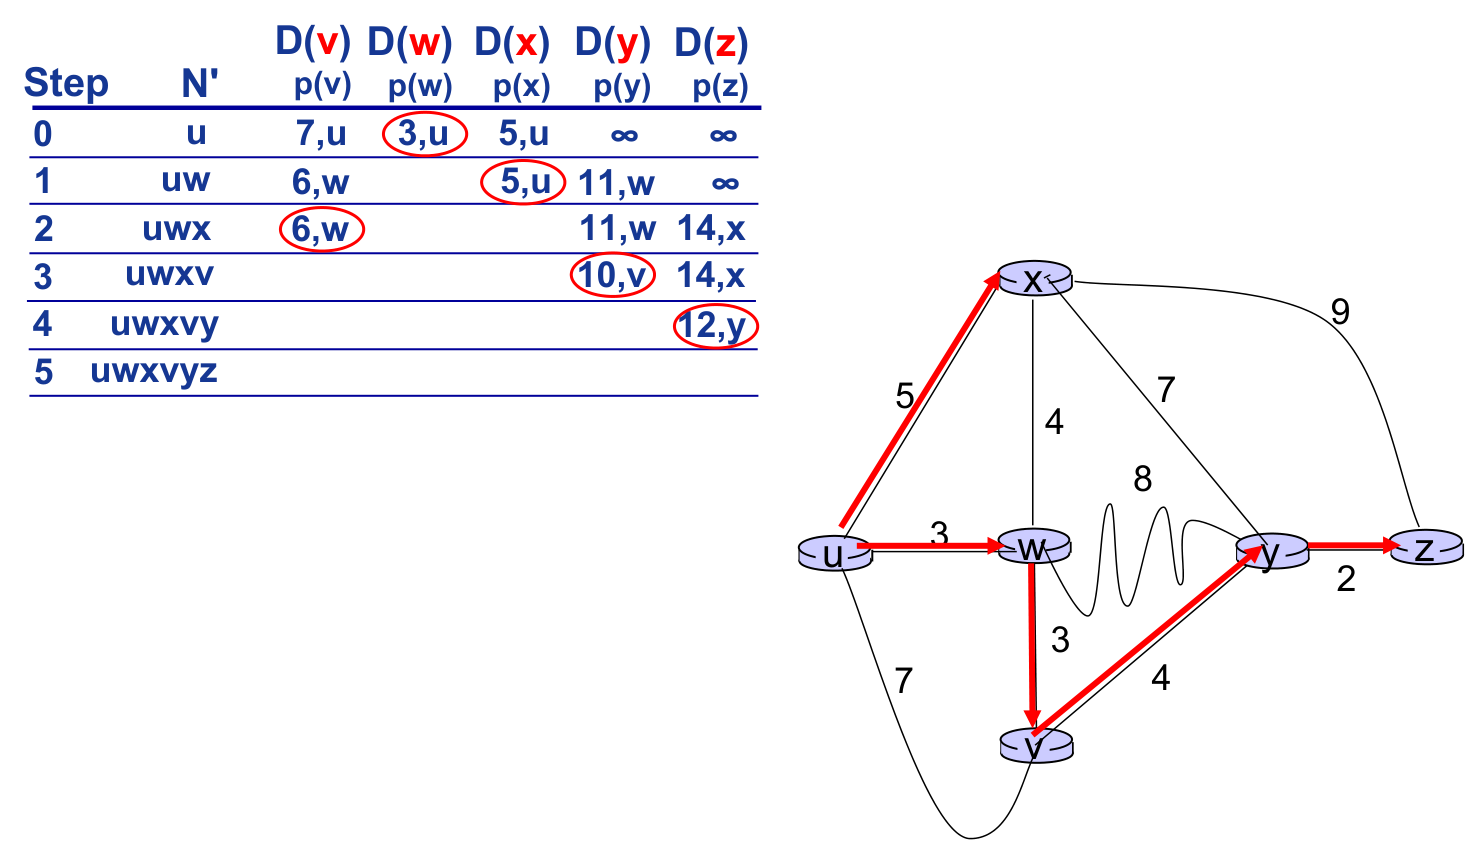
\includegraphics[width=.88\textwidth]{ch04-dijkstra.png}\caption{Dijkstra逐轮更新；左表记当前费用及前驱，右图中边上数字是费用。来源：Chapter4-网络层.pdf，PDF第155页（显示页155），局部截取。}\end{figure}
如果费用随流量改变且各路由器同步改路，负载可能在两条路径之间来回迁移，产生振荡。

\annotationarea[3]
\subsection{距离向量与无穷计数}
距离向量算法中，每个结点知道到邻居的链路费用，并向邻居通告自己到各目的地的距离估计。记 $D_x(y)$ 为结点 $x$ 估计到目的 $y$ 的费用，则收到邻居信息后更新
\[D_x(y)=\min_{v\text{为}x\text{的邻居}}\{c(x,v)+D_v(y)\}.\]
例如 $x$ 到 $y$ 为2、$y$ 到 $z$ 为1、$x$ 到 $z$ 直连为7；从 $y$ 得知其到 $z$ 为1后，$x$ 比较 $2+1=3$ 与7，选经 $y$ 的3。邻居继续交换后逐步收敛。

链路失效时，邻居可能仍保存旧距离，并错误地相互相信对方有通路；反复更新使费用逐渐增大，称\textbf{无穷计数}。\textbf{毒性逆转}要求某条路由若经邻居 $v$ 到达目的地，就向 $v$ 报告该目的不可达，能够阻止两结点互相依赖的部分环路，但不能消除所有多结点环路。限制最大度量也能使计数最终停止；例如RIP以16表示不可达。

\annotationarea[4]
\textbf{链路状态与距离向量的比较：}
\begin{center}\small\setlength{\tabcolsep}{3pt}
\begin{tabularx}{\textwidth}{>{\raggedright\arraybackslash}p{1.8cm}>{\raggedright\arraybackslash}X>{\raggedright\arraybackslash}X}
\toprule 比较点 & 链路状态（LS） & 距离向量（DV）\\\midrule
交换的信息 & 链路状态通告，汇集成网络拓扑 & 邻居之间交换到各目的地的距离估计\\
计算方式 & 每个路由器运行Dijkstra & 按Bellman--Ford方程反复更新\\
收敛与问题 & 计算量可为$O(n^2)$；费用随负载变动时可能振荡 & 收敛时间不定；可能有环路及无穷计数\\
错误传播 & 路由器通告错误链路费用，其他路由器各自计算自己的表 & 路由器通告错误路径费用，邻居可能继续据此更新并传播\\\bottomrule
\end{tabularx}\end{center}
\annotationarea[3]

\subsection{层次路由}
互联网规模大且由不同机构管理，把路由器组织成\textbf{自治系统 AS}。AS内路由协议决定系统内部路径；AS间协议交换外部前缀可达性，内部路由又确定到选定出口的路径。\textbf{热土豆路由}是在其他决策条件相同时，倾向选择本AS内部代价较低的出口；它不保证整个互联网端到端路径最短。
\par\small\noindent 来源：课件 PDF 第148--178页；教材 PDF 第197--199页（印刷第186--188页）。\normalsize

\annotationarea[4]
\section{路由协议}
\subsection{RIP：基于距离向量}
\textbf{RIP}（路由信息协议）是域内协议，以跳数作为度量；可达的最大度量为15，16表示不可达。相邻路由器周期性交换距离信息，课件给出常见周期30秒、约180秒未收到更新则视邻居失效；具体行为与实现和计时器有关。路由器比较“邻居报告的距离+到邻居的代价”，更新距离及下一跳。RIP采用UDP报文交换，跳数限制使其不适合很大的网络。

\textbf{课件例（PDF第182--183页）。} 路由器D当前到子网$w$经A为2跳，到$y$经B为2跳，到$z$经B为7跳，到$x$直连为1跳。若收到A的通告：A到$w$为1跳、到$x$为1跳、到$z$经C为4跳，且D到A的链路代价为1，则D重新比较：到$w$经A为$1+1=2$跳；到$x$经A为2跳但直连1跳更短；到$z$经A为$1+4=5$跳，比经B的7跳更短，故改成经A、5跳。此例展示DV的“邻居所报距离加本地链路费用，再取最小值”。

课件指出RIP表由应用进程route-d管理，周期性通告通过UDP数据报发送；收到并处理通告后，路由器据此更新转发表。\annotationarea[4]

\subsection{OSPF：链路状态与分区}
\textbf{OSPF}（开放最短路径优先）是域内链路状态协议：路由器泛洪链路状态信息，构建拓扑数据库，用Dijkstra计算路径；OSPF报文直接由IP承载。它可使用费用而非简单跳数，支持等价多路径及认证。

较大自治系统可分为多个\textbf{区域 area}和主干区域。区域内路由器掌握本区域详细拓扑；区域边界路由器连接区域与主干，并传播汇总信息；主干路由器在主干区运行OSPF，AS边界路由器负责与外部路由信息交互。区域减少拓扑信息扩散和计算规模；图中虚线包围不同区域，中间为主干。
\begin{figure}[H]\centering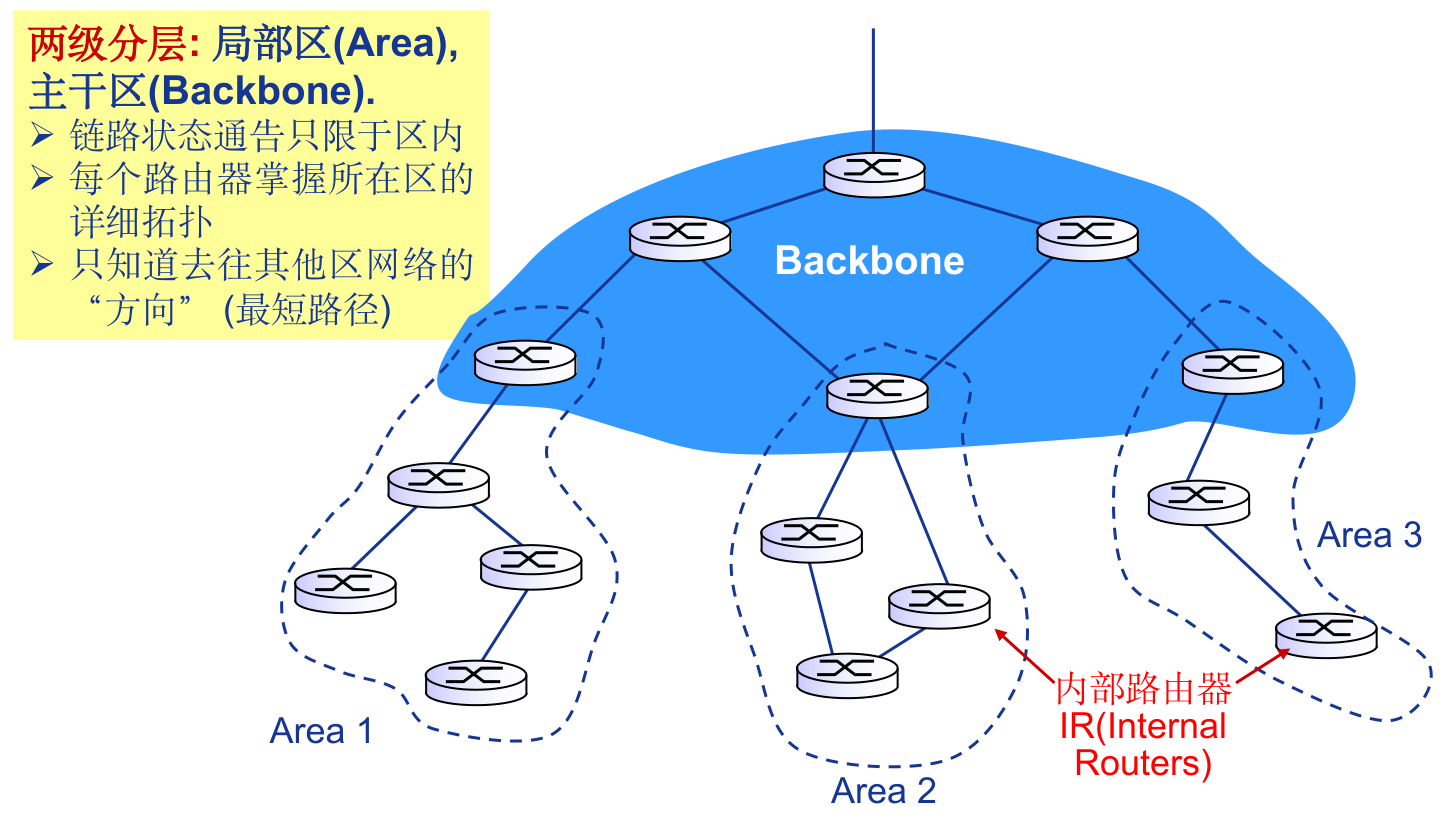
\includegraphics[width=.8\textwidth]{ch04-ospf-area.png}\caption{OSPF分区结构：区域经主干互连。来源：Chapter4-网络层.pdf，PDF第188页（显示页188），局部截取。}\end{figure}

\subsection{BGP：自治系统之间的策略路由}
\textbf{BGP}（边界网关协议）用于AS间交换目的前缀可达性；两个对等体通过TCP会话交换路径信息。eBGP在不同AS对等体间交换，iBGP在同一AS内部传播。路径通告包括\textbf{AS-PATH}（所经过的AS序列，可用于检测包含自身AS的环路）和\textbf{NEXT-HOP}（下一跳属性）。接收方可依据策略接受或拒绝，进而依据本地偏好、AS路径长度、到下一跳的内部代价等选择。策略优先于单纯的最短距离，不是每条学到的路由都会被再次通告。

BGP会话先建立TCP连接，再用OPEN协商参数；UPDATE通告或撤销路径，KEEPALIVE维持会话，NOTIFICATION报告差错并关闭会话。课件中的商业关系例表明：某AS未必愿意为两个非客户之间免费中转，故出口策略会限制可通告的路径。RIP、OSPF解决AS内部路由，BGP主要解决AS间可达性和策略。
\par\small\noindent 来源：课件 PDF 第180--200页；教材 PDF 第199--206页（印刷第188--195页）。\normalsize

\annotationarea[4]
\section{课件例题与综合练习详解}
\subsection{课件例2：链路状态算法Dijkstra的第二个算例}
从 $u$ 出发，课件 PDF 第156--157页给出另一组链路费用。按表格逐轮从未确定结点中选当前费用最小者，确定次序为 $u,x,y,v,w,z$；最终费用为 $D(v)=2$、$D(x)=1$、$D(y)=2$、$D(w)=3$、$D(z)=4$。例如 $u$ 到 $w$ 的路径是 $u\to x\to y\to w$，总费用 $1+1+1=3$；$u$ 到 $z$ 的路径是 $u\to x\to y\to z$，总费用 $1+1+2=4$。转发表记录第一跳：去往 $v$ 走 $(u,v)$，去往 $x,y,w,z$ 均先走 $(u,x)$。注意，费用表中的前驱结点与转发表中的下一跳不是同一概念：若前驱不是源结点，要沿前驱链回溯到源结点后的第一个结点。\annotationarea[4]

\subsection{课件例：距离向量的更新与链路失效}
课件 PDF 第163--164页的三结点例中，$x$ 到 $y$ 的链路费用为2，到 $z$ 的费用为7，$y$ 到 $z$ 的费用为1。$x$ 收到邻居通告后计算
\[
D_x(z)=\min\{c(x,y)+D_y(z),c(x,z)+D_z(z)\}=\min\{2+1,7+0\}=3,
\]
因此经 $y$ 到 $z$，而不是直连 $z$。\par
课件 PDF 第177--178页再给出R1--R2--R3线性拓扑。若到 $192.168.2.0/23$ 的已收敛跳数为 $(3,2,1)$，R3发现该网不可达后，R2尚保留旧消息，可能继续将R1的可达性误导到已断开的网络。第一轮交换后各路由器距离为 $(3,4,3)$；第二轮后为 $(5,4,5)$。因此题目问第二轮后R1的距离向量，答案是5跳。这个数字尚未表示网络已正确收敛，而是显示坏消息可能逐步增加度量。\annotationarea[4]

\subsection{课件例2：NAT端口映射}
课件 PDF 第135--138页的校园网中，R2后面的Web服务器是 $192.168.1.2$，外侧地址为 $203.10.2.2$；R3后面的H2地址也为 $192.168.1.2$，R3外侧地址为 $203.10.2.6$。两处相同的私有地址属于不同局域网。要让H2、H3访问Web默认端口，R2需静态映射
\[
203.10.2.2:80\longleftrightarrow 192.168.1.2:80.
\]
R3还须为内部主机配置出站NAT，使用R3的公网地址及端口区分会话。H2发出的HTTP数据报源IP为 $192.168.1.2$、目的IP为 $203.10.2.2$；R3做源地址转换后变为 $203.10.2.6\to203.10.2.2$；R2做目的地址转换后变为 $203.10.2.6\to192.168.1.2$。回包按相反次序查表改写。\annotationarea[4]

\subsection{课件例：从 /24 中分配三个局域网}
课件 PDF 第201--202页要求从地址块 $192.168.1.0/24$ 中划分三个局域网。已有子网 $192.168.1.0/25$ 已占用，剩余地址块为 $192.168.1.128/25$。三个局域网分别至少需要60、30、30个可用地址。\par
先给60台主机的网络分配/26：块大小64、可用62个；两个30台网络各分配/27：块大小32、可用30个。分配结果为：
\begin{center}\begin{tabular}{lllll}\toprule 局域网 & 网络/前缀 & 掩码 & 广播地址 & 可用地址范围\\\midrule
1 & $192.168.1.128/26$ & $255.255.255.192$ & $192.168.1.191$ & $192.168.1.129$--$192.168.1.190$\\
2 & $192.168.1.192/27$ & $255.255.255.224$ & $192.168.1.223$ & $192.168.1.193$--$192.168.1.222$\\
3 & $192.168.1.224/27$ & $255.255.255.224$ & $192.168.1.255$ & $192.168.1.225$--$192.168.1.254$\\\bottomrule\end{tabular}\end{center}
分配时先满足最大需求，并保证每个网络地址按块大小对齐；网络地址和广播地址不计入普通可用主机数。\annotationarea[4]

\subsection{课件例：为R1填写路由表并在R2聚合}
课件 PDF 第203--206页中，R1的E1、E2、E3、E4分别直连前三个新子网及已分配的 $192.168.1.0/25$；R1经L0到R2，下一跳地址为 $192.168.2.2$。相关路由项如下：
\begin{center}\begin{tabular}{llll}\toprule 目的网络 & 掩码 & 下一跳 & 接口\\\midrule
$192.168.1.128$ & $255.255.255.192$ & 直连 & E1\\
$192.168.1.192$ & $255.255.255.224$ & 直连 & E2\\
$192.168.1.224$ & $255.255.255.224$ & 直连 & E3\\
$192.168.1.0$ & $255.255.255.128$ & 直连 & E4\\
$201.18.3.0$ & $255.255.255.128$ & $192.168.2.2$ & L0\\
$201.18.3.254$ & $255.255.255.255$ & $192.168.2.2$ & L0\\
$0.0.0.0$ & $0.0.0.0$ & $192.168.2.2$ & L0\\\bottomrule\end{tabular}\end{center}
R2到达上述四个 $192.168.1.x$ 子网都经R1的 $192.168.2.1$、接口L0，因此可用 $192.168.1.0/24$ 聚合。能聚合的条件是地址前缀连续、下一跳和输出接口相同，而且汇总后不把本来不可达的地址错误地指向该下一跳；若误导流量就会形成路由黑洞。更具体路由可依最长前缀匹配覆盖汇总路由。\annotationarea[4]

\subsection{课件例：主机配置与错误掩码}
课件 PDF 第207--209页的例子中，H1位于 $201.18.3.0/25$。示例配置为IP地址 $201.18.3.1$、掩码 $255.255.255.128$；默认网关为 $201.18.3.126$，DNS服务器为 $201.18.3.254$。H1和DNS不在同一子网，因此主机把DNS查询交给默认网关。\par
H2的地址是 $201.18.3.2$。若它误用 $255.255.255.0$，就会把 $201.18.3.254$ 判断为本地链路上的主机，直接广播ARP询问服务器的MAC地址。H2所在的实际链路是 $201.18.3.0/25$，DNS服务器在另一子网，ARP广播不会通过路由器，因此解析失败，DNS查询也发不出去。正确的/25掩码使H2判断DNS服务器在异网，继而用ARP寻找默认网关MAC，再把DNS数据报交给路由器转发。\annotationarea[4]

\subsection{课件例：BGP出口选择}
课件 PDF 第173--199页说明，若同一前缀可由多个自治系统到达，路由器先依据本地偏好和策略决定接受哪些路径；之后可按AS-PATH长度、到NEXT-HOP的自治系统内费用等准则选择。热土豆路由是在可用外部路径中选择AS内部代价较低的网关，不保证端到端路径最短。提供商AS通常只向其他网络通告符合其商业策略的路径，例如不替两个非客户AS免费转发彼此的流量。\annotationarea[4]

\section*{本章自查：先自己回答，再对照解析}
\begin{enumerate}[nosep]
\item A到B跨越路由器时，B的IP地址是否每跳改变？帧目的MAC是否每跳都相同？
\item \texttt{192.168.1.130/26} 的网络地址、广播地址分别是什么？
\item IPv4数据报总长4000字节、首部20字节、MTU为1500字节时，第二片偏移是多少？
\item RIP与OSPF各与哪一种基本路由算法对应？BGP又主要用于什么范围？
\end{enumerate}
\textbf{参考答案：}1. 普通转发中目的IP不变；每段链路重新封装，目的MAC对应本跳接收接口，可改变。2. /26每块64个地址，130落在128--191，网络地址为 \texttt{192.168.1.128}，广播为 \texttt{192.168.1.191}。3. 第一片载荷1480字节，因此第二片偏移为 $1480/8=185$。4. RIP对应距离向量，OSPF对应链路状态；BGP主要用于自治系统之间的路由与策略。
\annotationarea[2]

